%!TEX root = ../main.tex


Enterprises and firewall
SBC and firewall traversal
Integration and interoperation

Necessary
Aims of the integration
Requirements


Suggestions about the integrated solution
Protcols
Network

Problems about the integrated solution


How can we integrate RTC in the Web with Virtual Arena?
There are two solutions to this problem the way I see it. The first is very obvious and complicated, but probably the best solution. The second is more of an experimental hack rather than a viable solution.

\section{The Gateway Solution}
The obvious solution is to create a gateway using \gls{wrtc} and Visual Arena to turn any \gls{wrtc} enabled browser into a client. The gateway will allow the web browser on your preferred device to make and receive connections from Virtual Arena. The gateway would have to contain three modules:
a Signaling Proxy, a Transport Proxy, and a Media Transcoder. The global architecture would look something like this:
\\
\\
\centerline{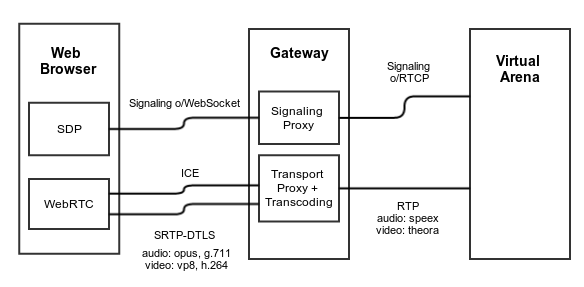
\includegraphics[scale=0.6]{gateway_architecture.png}}

\subsection{The Signaling Proxy}
Since \gls{wrtc} does not define any signaling protocol, one is free to use something custom made. But in this approach, the key information that needs to be exchanged is the \gls{sdp}, which specifies the necessary transport and media configuration information necessary to establish a connection. This approach is outlined by \gls{jsep}. So the role of the Signaling Proxy module would be to extend the custom signaling protocol already used in Virtual Arena to include the necessary metadata provided in the \gls{sdp}. It would go something lke this:

The \gls{mcu} sends an offer via the signaling method, then on the client the remote party would install it using the setRemoteDescription() API.

\begin{lstlisting}[frame=single]
...snip...
m=audio 1 RTP/SAVPF 111 103 104 0 8 106 105 13 126
c=IN IP4 0.0.0.0
a=rtcp:1 IN IP4 0.0.0.0
a=ice-ufrag:fAYfQM/iWMQPqiHs
a=ice-pwd:pgbuPPRdpKq+obC0lyRxVDe/
a=extmap:1 urn:ietf:params:rtp-hdrext:ssrc-audio-level
a=rtpmap:111 opus/48000/2
a=maxptime:60
a=ssrc:2209464108 cname:7oIEPieg3XZzHJdN
a=ssrc:2209464108 mslabel:uWu6kVvHhYbbkOtNalf5E2LFgjx4cpGMhnfo
a=ssrc:2209464108 label:2b626a18-c54c-4c1b-9f42-03519a9b63f2
m=video 1 RTP/SAVPF 100 116 117
...snip...
\end{lstlisting}

\subsection{The Transport Proxy}
The \gls{wrtc} specification make support for \gls{ice} and \gls{srtp}-{dtls} mandatory. The problem here is that Virtual Arena uses raw \gls{rtp} streams, it does not need the added security layers that \gls{wrtc} defines. It is up to the Transport Proxy to convert the media streams to allow these two worlds to interoperate. 

How can we take advantage of \gls{ice} and it's security? By modifying a constraint in the IceTransport object we can modify which candidates the ICE engine is allowed to use. We can indicate that the engine must use only relay candidates. This can be used to prevent leakage of IP addresses.


\subsection{The Media Transcoder}
The \gls{wrtc} specification defines these mandatory codecs:
\begin{itemize}
    \item Audio: opus and g.711
    \item Video: ?
\end{itemize}

There are still discussions on the topic of which video codec should be standard. The choice is between VP8 and H.264. The H.264 codec was recently made free by Cisco, so now both choices are royalty free. H.264 is the most widely deployed and currently has the best hardware support, but both Google and Firefox has decided to use VP8 in their WebRTC implementations.

Virtual Arena uses Speex for audio and Theora for video. So these would have to be transcoded to the appropriate formats.

This is one of the advantages of utilizing a \gls{mcu} because you can add support for both H.264 and VP8 and be able to create a session between  both Chrome, Virtual Arena, and Bowser.


\section{The Experimental Solution//TO DO}
A server that acts like a client. This could be done using the native client library. One problem with the native library is that it as far behind the web APIs in terms of development. This is because all the focus is on browser-to-browser scenarios. There are a couple of services out there that uses the native libraries, but most are commerce. There is one open-source solution that has the ability to create a server that acts like client, but we need more than that. We need to be able to attach remote incoming RTP streams to a peer connection. Signaling is already done on the server side so that should not be any different from the previous solution. What we need is one gateway server that can listen to UDP-packets from Virtual Arena and act as a peer in \gls{wrtc}. This is not an ideal approach, but pretty cool if it should work.

For a single person that acts as a PeerConnection in WebRTC to listen in on a conversation from Virtual Arena, one would need to initiate a fake RTC Connection using two peers, then create a MediaStream from the incoming UDP packets and inject that MediaStream into the RTC Connection. On the returning side one would have to take the MediaStreams and break them into pure RTC packets with an SSRC identifier in the header and send them in return to the \gls{mcu}.

First problem is receiving the incoming conversation from Virtual Arena this can be done setting up a socket that listens for incoming UDP packets. This is not a problem and can even be done in a pure Javascript environment using node.js

Then one would have to create a MediaStream Object from these packets. This is not currently possibly using chrome API's or Firefox. In chrome it is possible to create a pure audio MediaStream using the new WebAudio API, and in Firefox it should be possible to create a MediaStream from video using getStreamUntilEnded(), but this is currently broken. In the future however this should be possible using the drafted captureMedia APIs.

It is however possible to inject external MediaStreams into an RTC Connection.

For returning data from a PeerConnection to the \gls{mcu} on would have to record the stream and return the data over a an \gls{udp} connection. This should be done using the proposed MediaStream Recording APIs, but none of the browser have currently implemented these yet.